\subsection{Aplicação Fábrica: Menu Inicial}
\subsubsection*{Descrição do caso de uso}
No menu, espera-se que este seja muito simples e intuitivo. Deve conter botões que indiquem de forma inequívoca qual a qual funcionalidade dão acesso. As cores das opções já existentes na aplicação construida no Microsoft Access deverão ter cores similares.\\
Na primeira fase do projeto este menu deve apenas contemplar as opções existentes na aplicação anterior, tal como descrito na figura \ref{fig:di_fabrica_menu} a.\\
No final da segunda fase, espera-se que o menu inicial apenas acrescente dois botões no final, conforme demonstrado na figura \ref{fig:di_fabrica_menu} b

\begin{figure}[H]
	\centering
	
	\begin{subfigure}[t]{0.45\linewidth}
		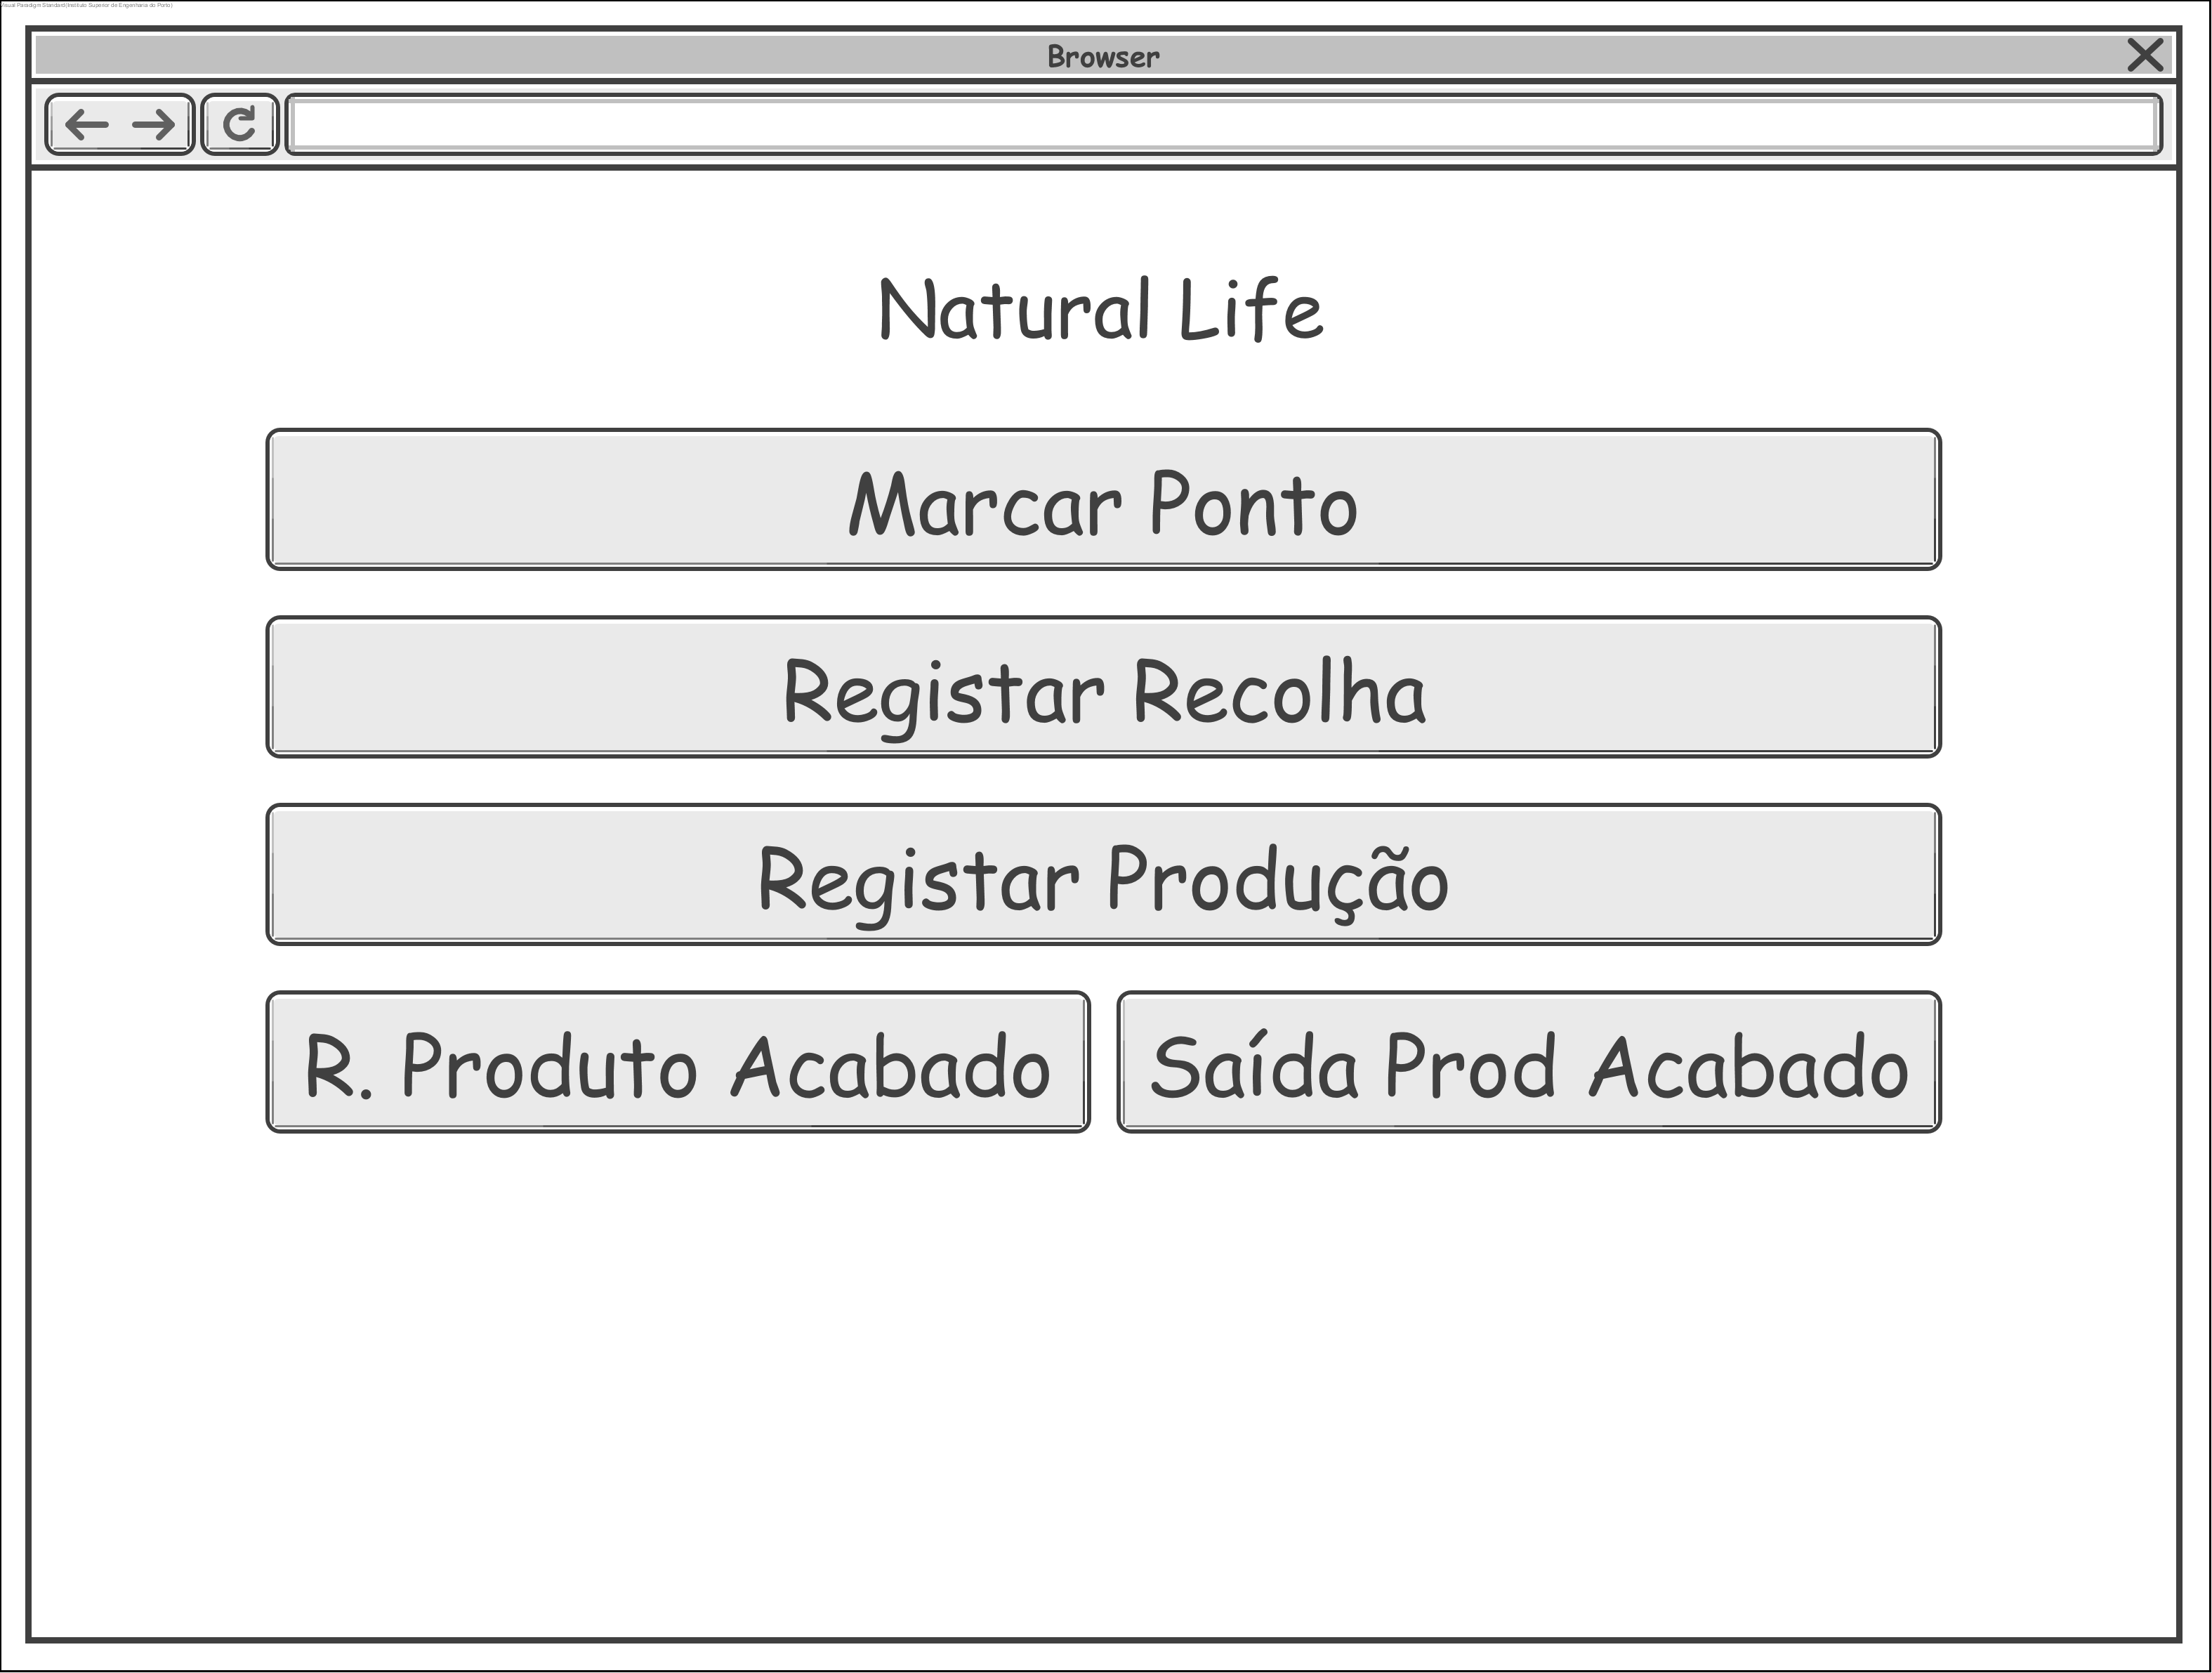
\includegraphics[width=\linewidth]{figuras/Diagramas_vp/DI_Fabrica_0-Menu_Inicial_-1a_Fase.png}
		\label{fig:di_fabrica_menu_1}
		\caption{Após concluir primeira fase}
	\end{subfigure}
	\begin{subfigure}[t]{0.45\linewidth}
		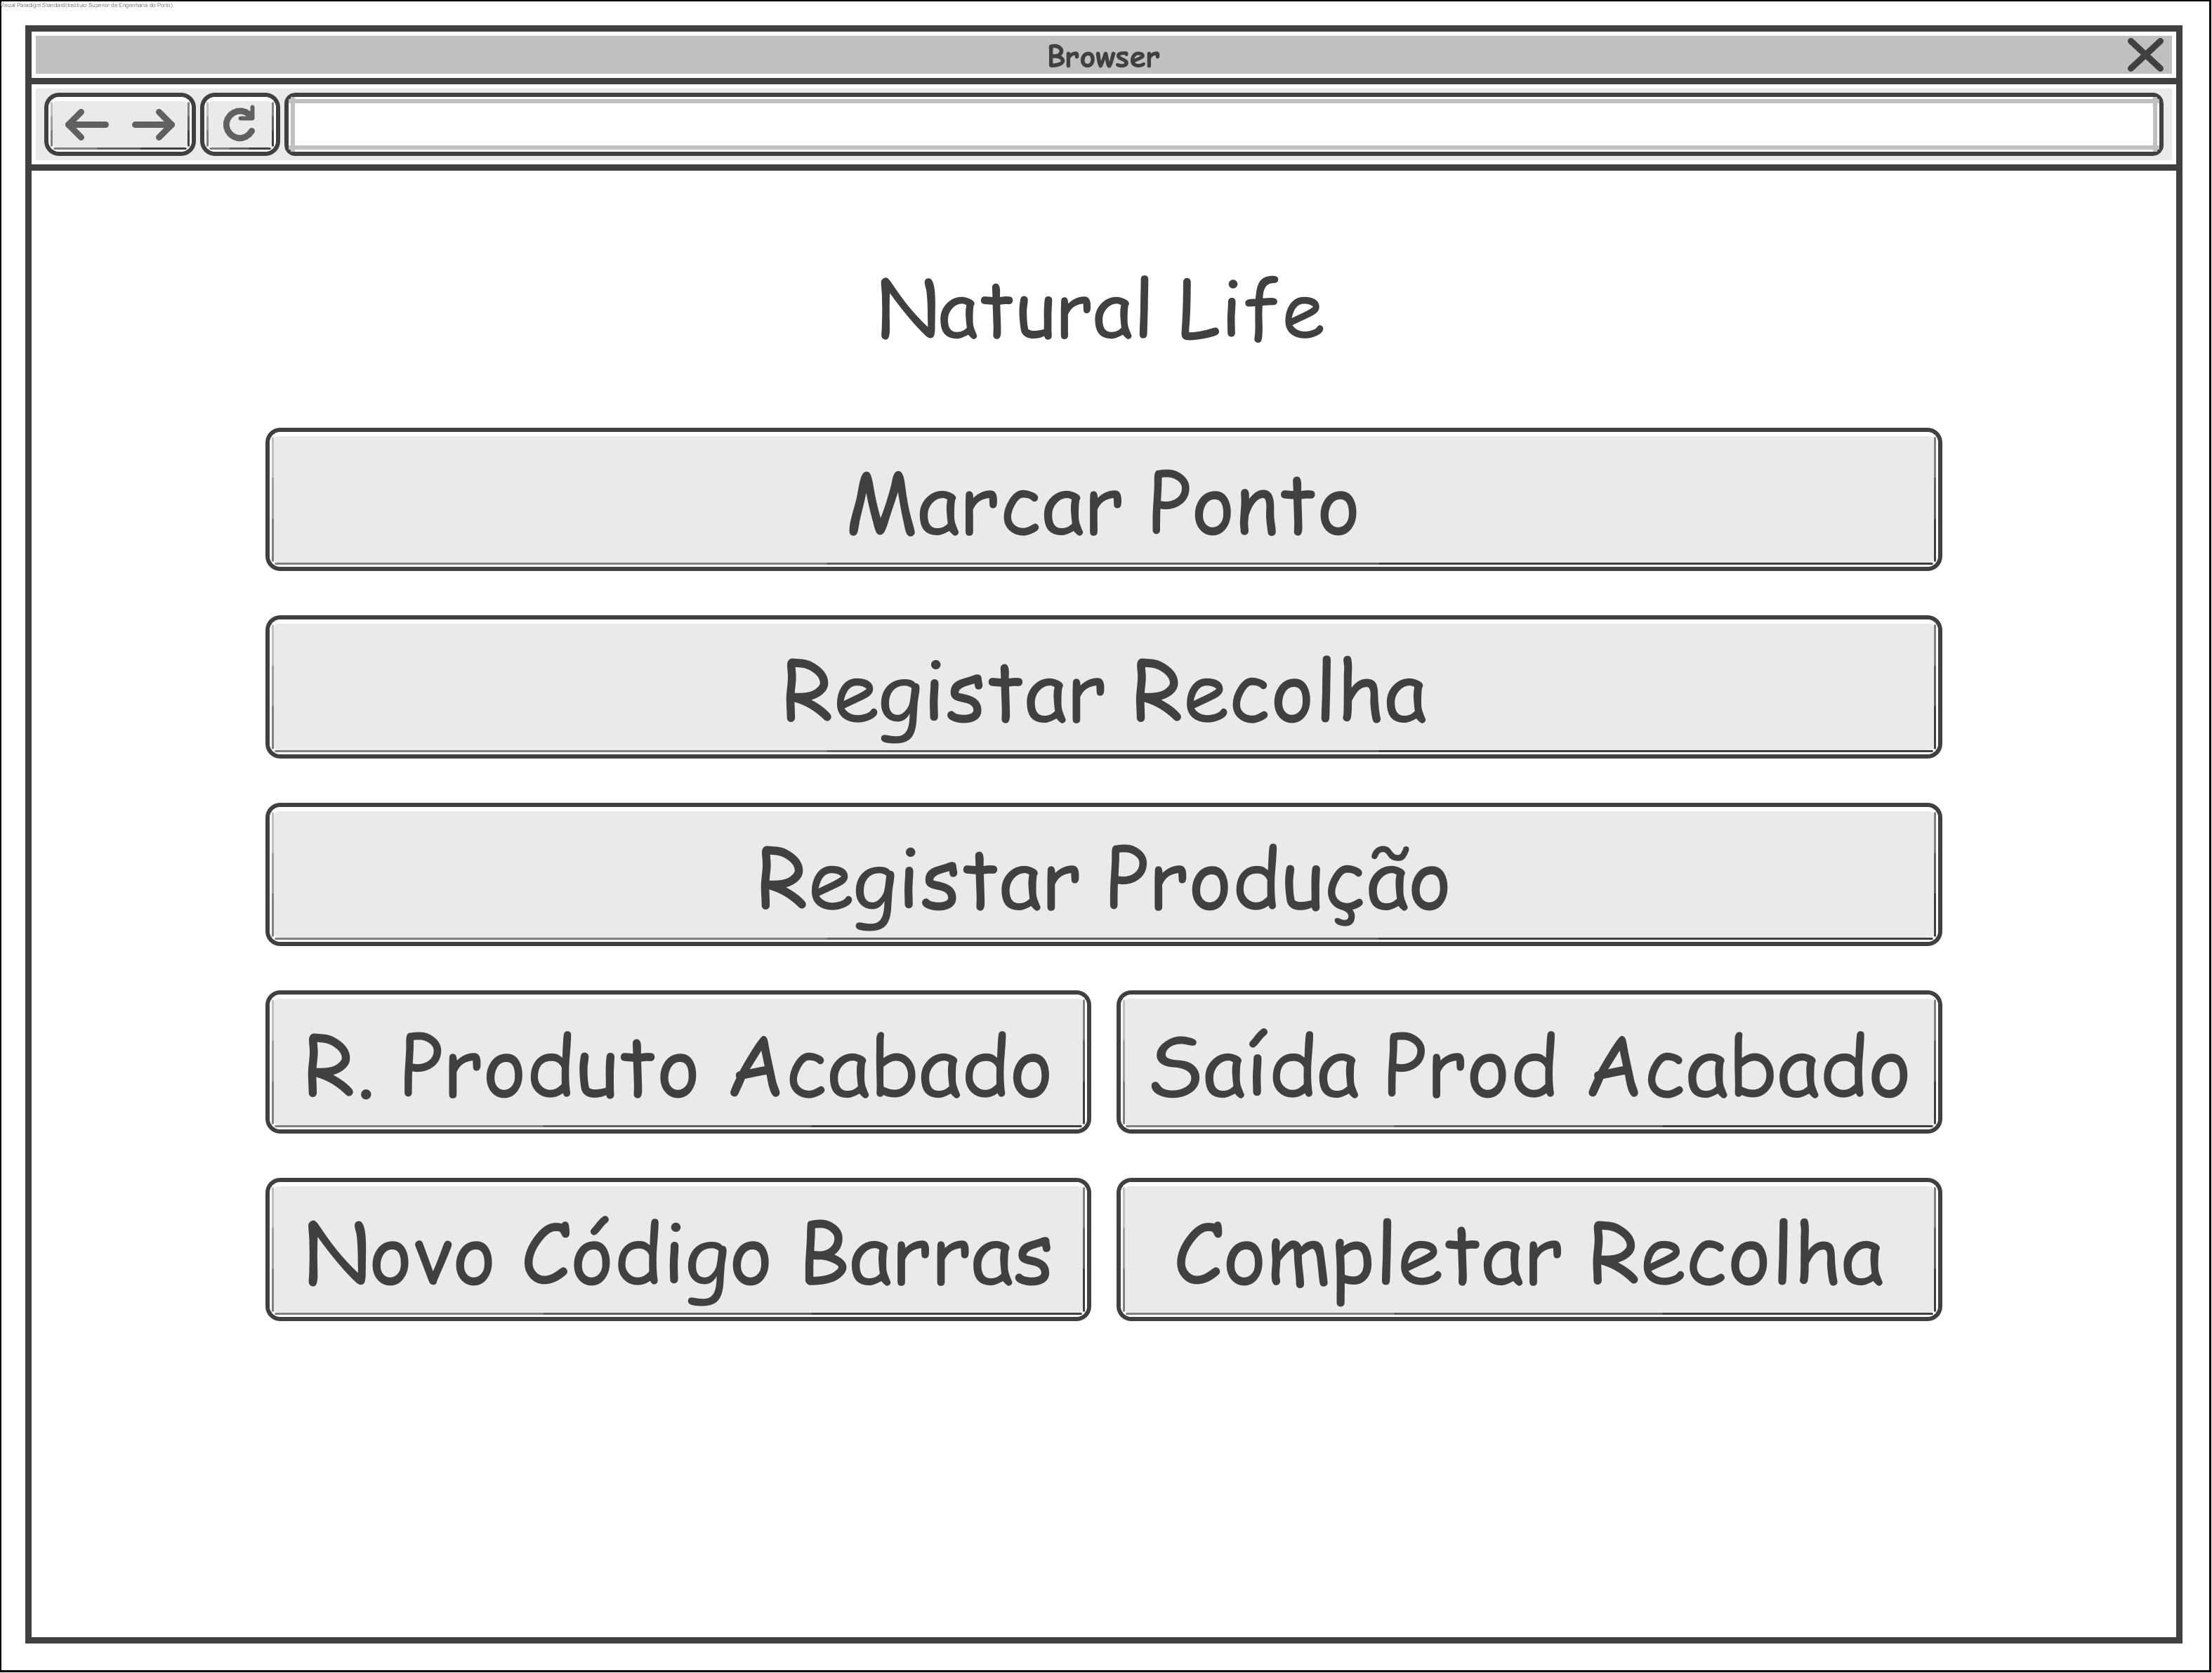
\includegraphics[width=\linewidth]{figuras/Diagramas_vp/DI_Fabrica_0-Menu_Inicial_-2a_Fase.png}
		\label{fig:di_fabrica_menu_2}
		\caption{Após concluir segunda fase}
	\end{subfigure}
	
	\caption{Modelo do menu}
	\label{fig:di_fabrica_menu}
\end{figure}